\section{Evaluation}
Our initial goal of having the grip classification being performed in real-time on the device was abandoned due to time constraints. Therefore we focused our evaluation criteria on how accurately the grip patterns could be identified. While training the model, we performed a 10-fold cross-validation that provides insight into the model's performance.

\subsection{Model Evaluation}
Table \ref{tbl-Grip Model Eval} demonstrates shows the performance of the model when trained with two datasets, and two algorithms - SMO and BayesNet. As expected, the prediction accuracy decreases when a larger dataset is used. This is due to the variability of the manner in which the gestures are performed. Conversely, this should also result in a more robust model that can accurately predict a gesture with small variations.

\begin{table}[!t]
\caption{Grip model cross validation accuracy with multiple datasets}
\label{tbl-Grip Model Eval}
\begin{tabular}{|l||l|l|l|l|l|l|}\hline
        & \multicolumn{3}{c|}{initial dataset} & \multicolumn{3}{c|}{expanded dataset} \\ \hline \hline
        & count     & SVM        & Bayes      & count     & SVM        & Bayes    \\
None    & 13751     & 99.4\%     & 98.8\%     & 20773     & 99.6\%     & 99.1\%      \\
Squeeze & 871       & 97.0\%     & 99.7\%     & 871       & 95.5\%     & 97.5\%      \\
Reach   & 679       & 97.9\%     & 99.3\%     & 1361      & 94.0\%     & 95.6\%    \\ \hline
\end{tabular}
\end{table}

It was determined that the best performance achieved by a model for the expanded dataset was using the J48 tree classifier, as shown in  Table \ref{tbl-Grip Model J48}. This makes intuitive sense since all the features are thresholded, which can be easily expressed as a \textit{classification tree}.

\begin{table}[!t]
\caption{J48 Grip model cross-validation Confusion Matrix}
\label{tbl-Grip Model J48}
\begin{tabular}{|l||l|l|l|l|l|}
\hline
        & total & None  & Squeeze & Reach & Correct \\ \hline \hline
None    & 20773 & 20729 & 9       & 35    & 99.8\%  \\
Squeeze & 871   & 9     & 855     & 7     & 98.2\%  \\
Reach   & 1361  & 16    & 4       & 1341  & 98.5\%  \\ \hline
\end{tabular}
\end{table}


\subsection{Off-line Evaluation}
We decided to use the J48 tree grip detection model since it produced the best cross-validation results. Since we are not performing real-time evaluation, we first record our evaluation dataset in a manner similar to the training dataset - generating a log of the sensor values as the user performs the squeeze and reach gestures. This dataset is then parsed to generate the sliding windows and extract the features.
\par
We wrote a simple Java program running on a laptop that would load the J48 grip classification model, read the features of each window and ask the model to classify it as None, Squeeze or Reach gesture. Without looking at the predictions for each window, we classified each window manually. Figure \ref{fig:reach_eval} and Figure \ref{fig:squeeze_eval} displays a comparison of the predicted and actual window classifications for Reach and Squeeze grips, respectively. The average difference between the classifications was 2\% on average, with a maximum of 6\%, for both types of gestures.
\par
Similar to tap detection, a gesture is detected when 50 consecutive windows are classified as the same. It was observed that the misclassified windows all tended to be at the beginning or the end of each gesture duration. For each of the Squeeze or Reach gestures, there was always a set 50 consecutive windows that were correctly classified. This means that the gestures were detected with 100\% accuracy.

\begin{figure}[h]
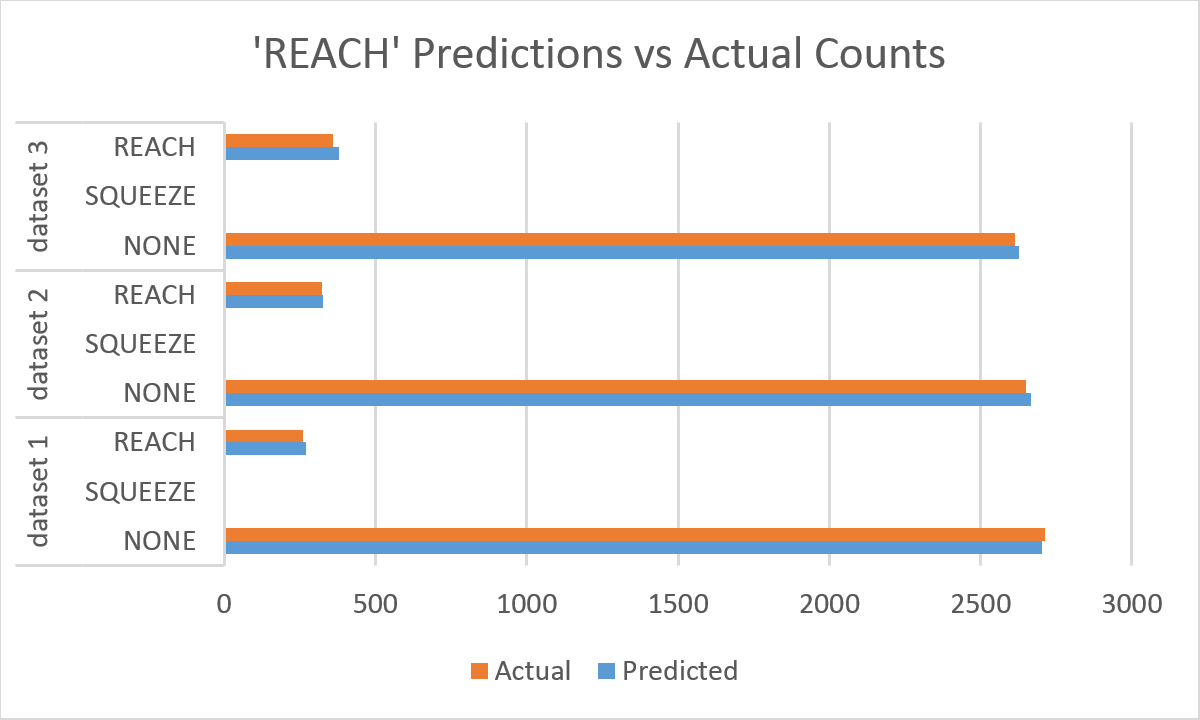
\includegraphics[width=.45\textwidth]{reach_eval.png}
\caption{'Reach' grip evaluations for 3 distinct datasets}
\label{fig:reach_eval}
\end{figure}


\begin{figure}[h]
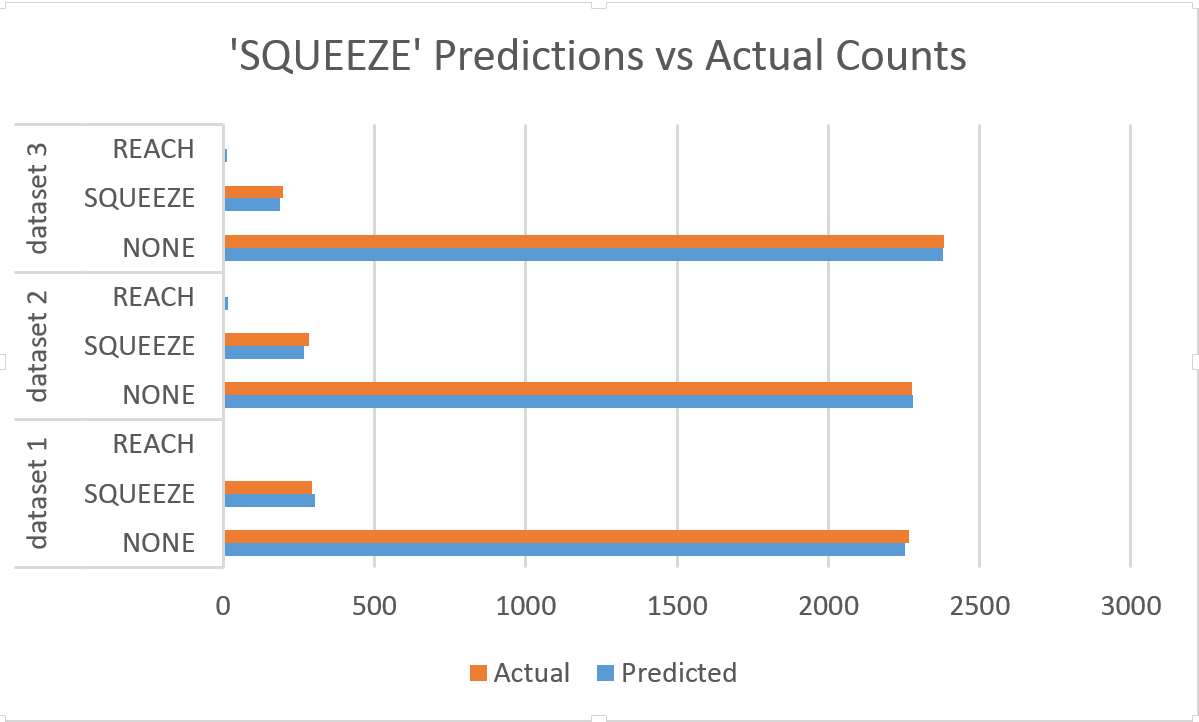
\includegraphics[width=.45\textwidth]{squeeze_eval.png}
\caption{'Squeeze' grip evaluations for 3 distinct datasets}
\label{fig:squeeze_eval}
\end{figure}

